\documentclass{beamer}

\usepackage{graphicx}
\usepackage{booktabs}
\usepackage{hyperref}
\usepackage{url}
\usepackage{listings}
\usepackage{verbatim}

\usetheme{Madrid}
\setbeamertemplate{navigation symbols}{}

\title{Matlab Usage Statistics}
\author{Akshay Khadse \and Raghav Gupta}
\institute[IITB]
{Indian Institute of Technology, Bombay}
\date{\today}

\begin{document}

\begin{frame}
    \titlepage
\end{frame}

\begin{frame}
    \frametitle{Overview}
    \tableofcontents
\end{frame}


\section{Special Packages}
\subsection{Plotly}
\begin{frame}
    \frametitle{Plotly}
    \textbf{Features}
    \begin{itemize}
        \item Interactive Plotting Library
        \item Supports bar, line, scatter, maps and many more
        \item Supports online, offline plotting
        \item Allows styling in Python
    \end{itemize}
    \textbf{Why Plotly?}
    \begin{itemize}
        \item Offline plotting is easy
        \item Allows export to HTML div tag
        \item No other javascript dependencies
    \end{itemize}
\end{frame}

\subsection{LDAP3}
\begin{frame}
    \frametitle{LDAP3}
    \begin{itemize}
        \item LDAP operations are clumsy
        \item \texttt{python-ldap} module works with Python2
        \item \texttt{ldap3} developed in Python3 native, works for both
        \item Simplified Query Construction
        \item Allows secured access
        \item Conforms to current standards
    \end{itemize}
\end{frame}

\subsection{Django}
\begin{frame}
    \frametitle{Django}
    \textbf{Features}
    \begin{itemize}
        \item Django is a high-level Python Web framework
        \item Takes care of much of the hassle \\eg. authentication, site maps, RSS feeds etc
        \item Fast, Secure and Scalable
        \item Shortucts for common tasks
    \end{itemize}
    \textbf{Why Django?}
    \begin{itemize}
        \item Project has institute level scope
        \item Reusable apps can be used by other projects easily
        \item Good learning opportunity
    \end{itemize}
\end{frame}

\section{Git}
\begin{frame}
    \frametitle{Git}
    \url{https://www.github.com/akshaykhadse/matlab-usage-stats/}
    \begin{figure}
        \centering
        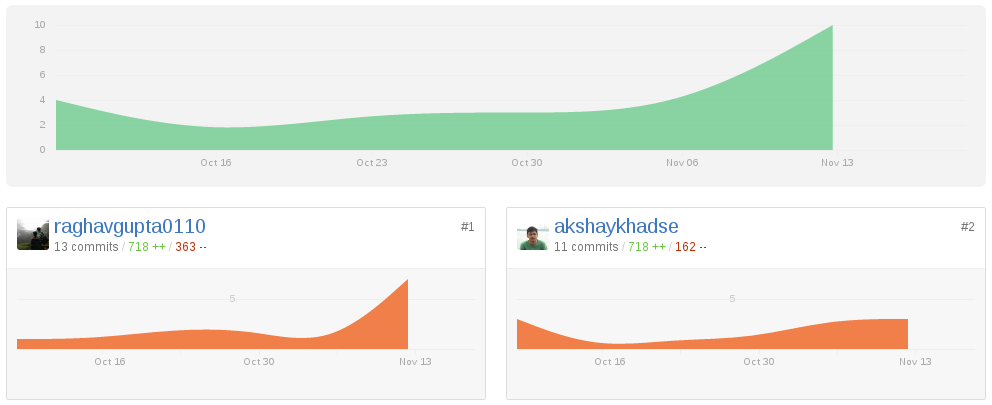
\includegraphics[scale=0.35]{github}
    \end{figure}
\end{frame}

\section{Continous Integration}
\begin{frame}
    \frametitle{Continous Integration}
    \textbf{Travis CI}
    \begin{itemize}
        \item Installs Dependencies
        \item Runs tests
        \item Checks PEP8
    \end{itemize}
    \textbf Coveralls
    \begin{itemize}
        \item 99\% coverage
        \item Tried to test every bit of code authored by us
        \item Django setup code ignored
        \item Non Runnable code ignored
    \end{itemize}
\end{frame}

\section{Documentation}
\begin{frame}
    \frametitle{Documentation}
    \begin{itemize}
        \item Docs hosted at \url{https://matlab-usage-stats.readthedocs.io/}
        \item Based on Sphinx, ReST
        \item Provided Docstrings for models, views and forms
        \item Non app processing functions also included
    \end{itemize}
\end{frame}

\section{Tests}
\begin{frame}
    \frametitle{Tests}
    \begin{itemize}
        \item Used unittests and mock
        \item \textbf{Models}
        \begin{itemize}
            \item Tested Object Creation
            \item Object saving and querying
        \end{itemize}
        \item \textbf{Views}
        \begin{itemize}
            \item Tested Context
            \item Tested response content
        \end{itemize}
        \item \textbf{django.test.Client} allows makeing requests like browser
        \item \textbf{Forms}
        \begin{itemize}
            \item Not Tested
            \item Testing views covers forms
        \end{itemize}
    \end{itemize}
\end{frame}

\section{Working}
\begin{frame}
    \frametitle{How to use?}
    \begin{itemize}
        \item Download zip from repo
        \item \texttt{\$ python3 setup.py install}
        \item Move log files into \texttt{data} folder in project root
        \item \texttt{\$ python3 manage.py runserver}
    \end{itemize}
\end{frame}

\subsection{List View}
\begin{frame}
    \frametitle{List View}
    On request, all entries are fetched from DB rendered on template for table and sent back as response.
    \begin{figure}
        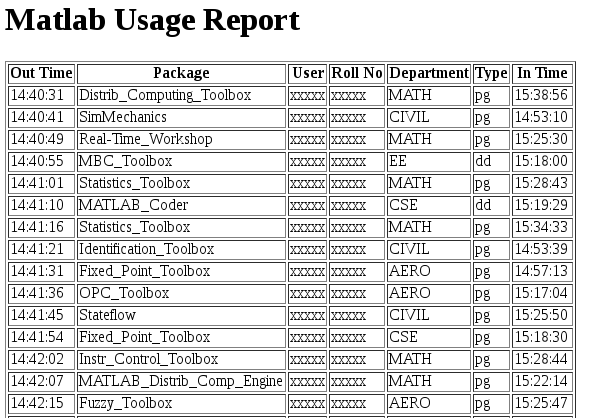
\includegraphics[scale=0.45]{listview}
        \caption{List View}
    \end{figure}
\end{frame}

\subsection{Graph View}
\begin{frame}
    \frametitle{Graph View}
    On request, all entries are fetched from DB, plotly graph is generated and sent back as response.
    \begin{figure}
        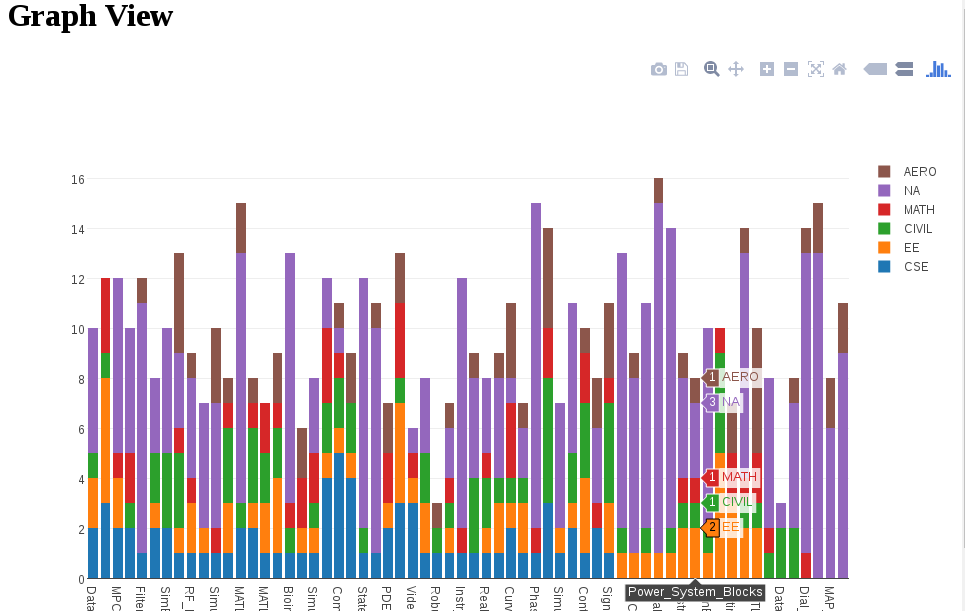
\includegraphics[scale=0.32]{graphview}
        \caption{Graph View}
    \end{figure}
\end{frame}

\subsection{Departments View}
\begin{frame}
    \frametitle{Departments View}
    If form is submitted, all entries from selected department are fetched from DB, plotly graph is formed and sent back as response.
    \begin{figure}
        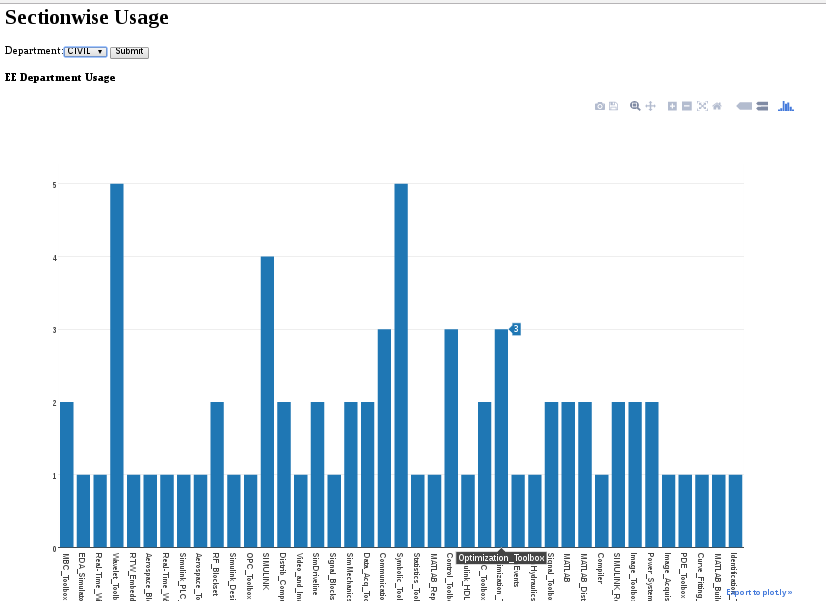
\includegraphics[scale=0.35]{departmentview}
        \caption{Department View}
    \end{figure}
\end{frame}

\subsection{Time View}
\begin{frame}
    \frametitle{Time View}
    If form is submitted, all entries from selected time frame are fetched from DB, plotly graph is formed and sent back as response.
    \begin{figure}
        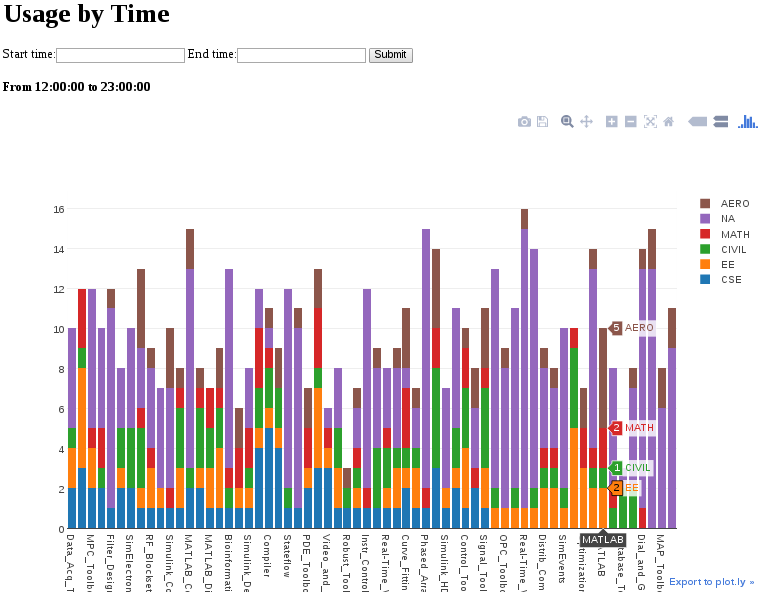
\includegraphics[scale=0.35]{timeview}
        \caption{Time View}
    \end{figure}
\end{frame}

\begin{frame}[fragile]
    \frametitle{Issues}
    \begin{block}{Excluding from Coverage}
        \begin{itemize}
            \item \texttt{coverage run --rcfile=.coveragerc manage.py test parser reports}
            \item \texttt{.coveragerc}
            \begin{verbatim}
omit =
    */__init__.py
    reports/apps.py
exclude_lines =
    if __name__ == .__main__.:
    \end{verbatim}
        \end{itemize}
    \end{block}
\end{frame}

\begin{frame}[fragile]
    \frametitle{Issues}
    \begin{block}{Testing LDAP}
        \begin{itemize}
            \item Testing \texttt{ldap\_search} by mock
            \begin{verbatim}
@mock.patch('parser.ldap_search.Connection')
class Test_ldap_search(TestCase):
    def test_ldap_search(self, mock_connection):
        ...
        expected = [mock.call('ldap.iitb.ac.in',
                              auto_bind=True),
                    mock.call().search(basedn, query,
                                       attributes=attrs)]
        mock_connection.assert_has_calls(expected)
    \end{verbatim}
        \end{itemize}
    \end{block}
\end{frame}


\begin{frame}
    \frametitle{Future Scope}
    \begin{itemize}
        \item \textbf{Synchronous Queue Processing}\\Process of updating database from logs is manual\\This can be periodically automated with RabbitMQ and Celery
        \item \textbf{Revamping Interface}\\Present web interface is plain html.\\Ignored due to out of subject's scope.\\Templating using Bootstrap would take very little effort
        \item \textbf{Extension to other license servers}\\Other could be included based on similar strategy.
    \end{itemize}
\end{frame}

\end{document}
